\documentclass[8pt]{beamer}
\usepackage{tikz}
\usepackage[utf8]{vietnam}
\usepackage{amsmath}
\usepackage{graphicx}
\usepackage{wrapfig}
\usepackage{hyperref}
\usetheme{Copenhagen}
\usecolortheme{beaver}
\setbeamertemplate{navigation symbols}{}
\setbeamertemplate{headline}{}
\title[Chương 2: Hệ thống LTI] %optional
{Chương 2: Hệ thống LTI}
\subtitle{Tín hiệu và hệ thống}
\author[Tín hiệu và hệ thống] % (optional)
{Tín Vũ}
\date[VLC 2021] % (optional)
{tinvu1309@gmail.com}
\begin{document}
\frame{\titlepage}
\begin{frame}{Mục lục}
\tableofcontents
\end{frame}
\begin{frame}{Giới thiệu playlist}
\section{Giới thiệu playlist}
	\begin{itemize}
		\item Mình là Tín Vũ, hiện tại đang là sinh viên học tại Trường Đại học Công nghệ, Đại học Quốc gia Hà Nội. Mình tạo playlist video này để hỗ trợ các bạn học môn Tín hiệu và hệ thống trong các trường đại học kĩ thuật theo hướng \alert{trực quan hóa} nhất có thể.
		\item Do đó, mục tiêu của mình khi thực hiện playlist này không chỉ giúp các bạn ôn thi được điểm cao mà còn \alert{hiểu sâu công thức để làm nền tảng cho các môn học sau}.
		\item Để đạt được hai mục tiêu trên, các bạn nên xem \textbf{toàn bộ} video của mình, còn nếu chỉ cần ôn thi cấp tốc và đạt điểm cao thì hãy \textbf{bỏ qua} các video "optional".
		\item Nội dung playlist này chủ yếu bám sát nội dung môn học Tín hiệu và hệ thống tại trường của mình; nếu các bạn học trường khác, hãy tham khảo kĩ đề cương hay đề thi của trường bạn để đối chiếu sao cho ôn tập đúng trọng tâm và hợp lý. 
		\item Môn học này bao gồm \textbf{6} chương, các chương đều liên quan rất chặt chẽ và logic với nhau nên hãy học cẩn thận ngay từ \alert{chương 0} để ôn thi cuối kì đỡ vất vả.
	\end{itemize}
\end{frame}
\begin{frame}{Tài liệu tham khảo}
\section{Tài liệu tham khảo}
\begin{itemize}
		\item Tài liệu tham khảo chính: Signals and Systems (2nd edition) Alan V. Oppenheim and Alan S. Willsky.
		\item Tài liệu tham khảo phụ: Bài tập của mình học khóa trước, đề thi các năm cũ,...
		\item Tài liệu tham khảo phụ: Nếu bạn là sinh viên trường mình và muốn học "tủ" nhiều bài thì nên đọc Signals and Systems (2nd edition) Simon Haykin vì các thầy cô chủ yếu dạy và ra đề trong cuốn này, thế nhưng mình đánh giá cuốn này không đầy đủ và chi tiết như sách của Alan V. Oppenheim. 
	\end{itemize}
\end{frame}
\begin{frame}{Khái niệm hệ thống LTI}
\section{Khái niệm hệ thống LTI}
Trong \alert{Chương 1}, chúng ta đã làm quen và khảo sát $5$ tính chất cơ bản của hệ thống gồm: \textbf{tính nhân quả}, \textbf{tính không nhớ}, \textbf{tính ổn định}, \alert{tính tuyến tính} và \alert{tính bất biến}. Từ \alert{Chương 2} trở đi cho đến hết môn học này, chúng ta sẽ tập trung khảo sát một họ hệ thống có \textbf{tính tuyến tính} (linear time) và \textbf{tính bất biến} (invariant), hay còn gọi là \alert{hệ thống LTI}.
\\ Suy ngẫm: tại sao chúng ta lại quan tâm đặc biệt đến hệ thống LTI ? Theo bạn, có phải là do đa số các hệ thống vật lý đều tuân theo \textbf{nguyên lý chồng chất (superposition)} không ? Bạn hãy thử tìm ví dụ minh họa cho các hệ thống vật lý có/không có tính tuyến tính.
\\ Tương tự như \alert{Chương 1}, chúng ta cũng phân loại hệ thống LTI gồm \textbf{hệ thống LTI liên tục} và \textbf{hệ thống LTI rời rạc}. Ngoài cách biểu diễn hệ thống bằng \textbf{phương trình đầu vào-ra} tổng quát với tất cả các loại hệ thống đã học ở chương trước, hệ thống LTI còn có thể được biểu diễn bằng \textbf{đáp ứng xung của hệ thống}.
\end{frame}
\begin{frame}{Biểu diễn hệ thống LTI bằng đáp ứng xung}
\section{Biểu diễn hệ thống LTI bằng đáp ứng xung}
\subsection{Hệ thống LTI rời rạc}
\subsubsection{Tích chập rời rạc}
\begin{itemize}
	\item Hệ thống LTI rời rạc
\end{itemize}

\begin{itemize}
	\item[-] Tích chập rời rạc
\end{itemize}
Trong toàn bộ $6$ chương của môn học, đây là phần kiến thức duy nhất chúng ta sẽ xây dựng khái niệm và tiếp cận từ tín hiệu/hệ thống rời rạc trước do tích chập rời rạc tương đối dễ hiểu hơn tích chập liên tục. Chúng ta bắt đầu từ một tín hiệu liên tục $x(t)$ được \textbf{lấy mẫu} thành tín hiệu rời rạc $x[n]$ như hình minh họa:
 \begin{figure}[h]
			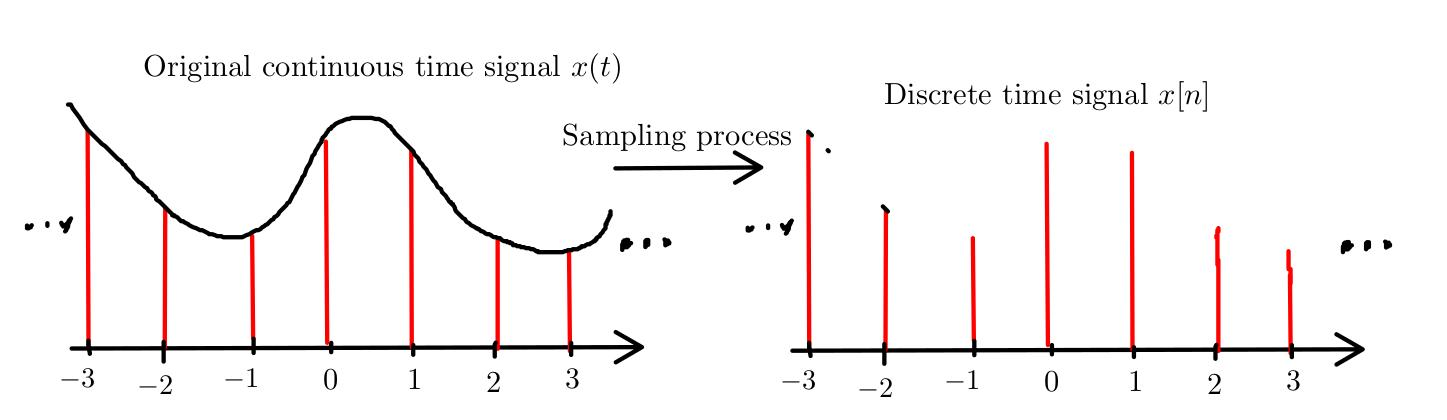
\includegraphics[width=0.6\textwidth]{discrete.jpg}
			\caption{Sampling process}			\label{fig:re1}
		\end{figure}
Như đã thảo luận ở \alert{Chương 1}, chúng ta có thể biểu diễn dữ liệu của chuỗi $x[n]$ như sau:
\begin{equation*}
	\begin{cases}
		\dots \\
		x[-2]=0.65\\
		x[-1]=0.4\\
		x[0]=0.9\\
		x[1]=0.96\\
		\dots \\
	\end{cases}
\end{equation*}
\end{frame}
\begin{frame}{Biểu diễn hệ thống LTI bằng đáp ứng xung}
	Cách biểu diễn chuỗi dữ liệu $x[n]$ như trên không tiện về mặt toán học do tương đối cồng kềnh và khó xử lý, chúng ta muốn tìm một cách biểu diễn $x[n]$ gọn hơn bằng \textbf{tổng vô hạn} như sau:

 \begin{figure}[h]
			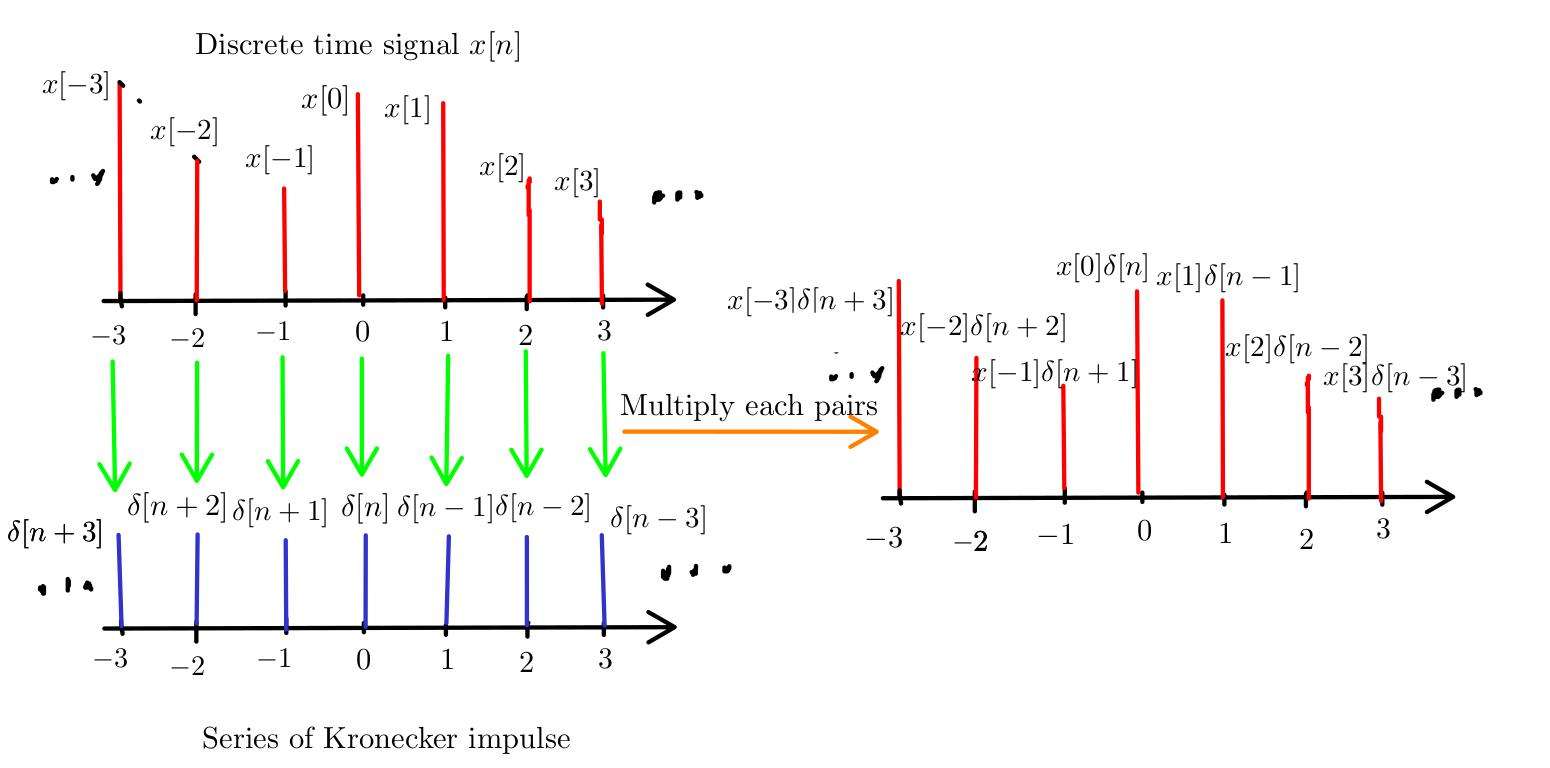
\includegraphics[width=1\textwidth]{process.jpg}
			\caption{Running sum visualization}\label{fig:re2}
		\end{figure}
\end{frame}
\begin{frame}{Biểu diễn hệ thống LTI bằng đáp ứng xung}
Từ hình minh họa trên, chúng ta thu được công thức biểu diễn $x[n]$ tổng quát bằng \textbf{tổng vô hạn} như sau:
\begin{block}{Công thức biểu diễn tín hiệu $x[n]$ tổng quát}
	$$x[n]=\sum_{k=-\infty}^{+\infty}x[k]\delta[n-k]$$
\end{block}
Suy ngẫm: tại sao tổng này còn được gọi là "running sum" ? Bạn hãy thử biểu diễn lại công thức trên và quan sát "cái gì" đang "chạy" ?
\\ Chúng ta tiếp tục cho tín hiệu đầu vào $x[n]$ trên đi qua một hệ thống LTI rời rạc có \alert{đáp ứng xung $h[n]$} (tạm thời bạn chưa cần hiểu khái niệm này, cứ công nhận trước đã), ta thu được tín hiệu ra $y[n]$ như sau:
\begin{figure}[h]
			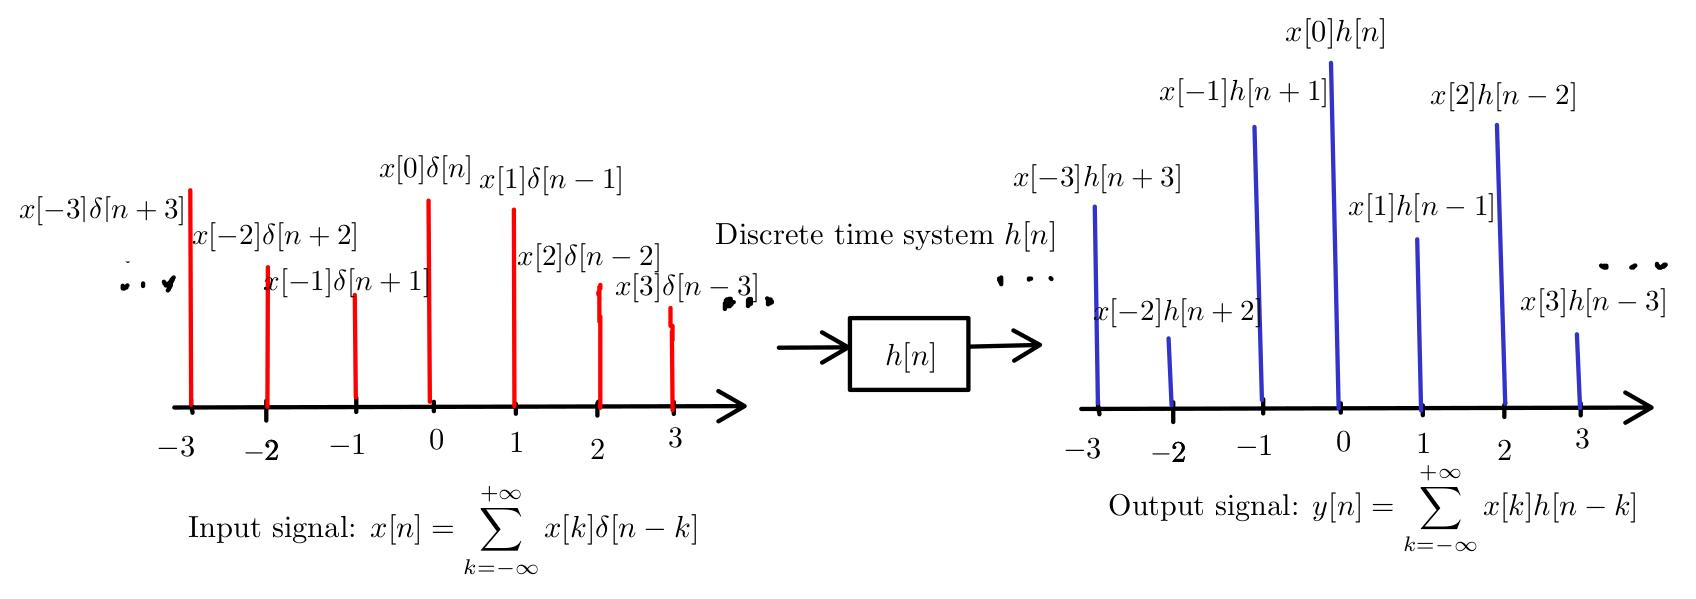
\includegraphics[width=0.8\textwidth]{system.jpg}
			\caption{In/output of LTI discrete time system}\label{fig:re3}
		\end{figure}
\end{frame}
\begin{frame}{Biểu diễn hệ thống LTI bằng đáp ứng xung}
	Quan sát tín hiệu ra $y[n]$, chúng ta nhận thấy hệ thống LTI rời rạc đã làm \textbf{biến đổi các thành phần $\delta[n-k]$ trong tín hiệu lối vào thành $h[n-k]$ ở tín hiệu lối ra}. Vậy ta có công thức biểu diễn tín hiệu $y[n]$ tổng quát (đầu ra của hệ thống LTI rời rạc) theo $x[n]$ (đầu vào của hệ thống LTI rời rạc) như sau:
	\begin{block}{Công thức biểu diễn tín hiệu $y[n]$ tổng quát}
		$$y[n]=\sum_{k=-\infty}^{+\infty}x[k]h[n-k]=\alert{x[n]*h[n]}$$
	\end{block}
	Toán tử $*$ được gọi là \alert{tích chập} (convolution). Vậy \alert{tích chập} là phép toán dùng để \textbf{tìm tín hiệu đầu ra $y[n]$ khi đã biết tín hiệu đầu vào $x[n]$ và đáp ứng xung của hệ thống LTI $h[n]$ }.
	\\ Suy ngẫm: xét tín hiệu đầu vào $x[n]=\delta[n]$ qua một hệ thống LTI $h[n]$. Tín hiệu ra $y[n]$ tức là đáp ứng của hệ thống với đầu vào là xung Kronecker (đáp ứng xung) có công thức như thế nào ? Bạn đã hiểu lý do tại sao $h[n]$ được gọi là \textbf{đáp ứng xung} của hệ thống chưa ?
	\\ Ví dụ: Cho một tín hiệu $x[n]=\alpha^{n}u[n]$ với $0<\alpha<1$ đi qua hệ thống LTI rời rạc có đáp ứng xung $h[n]=u[n]$, xác định tín hiệu ra của hệ thống.
\end{frame}
\begin{frame}{Biểu diễn hệ thống LTI bằng đáp ứng xung}

\begin{figure}[h]
			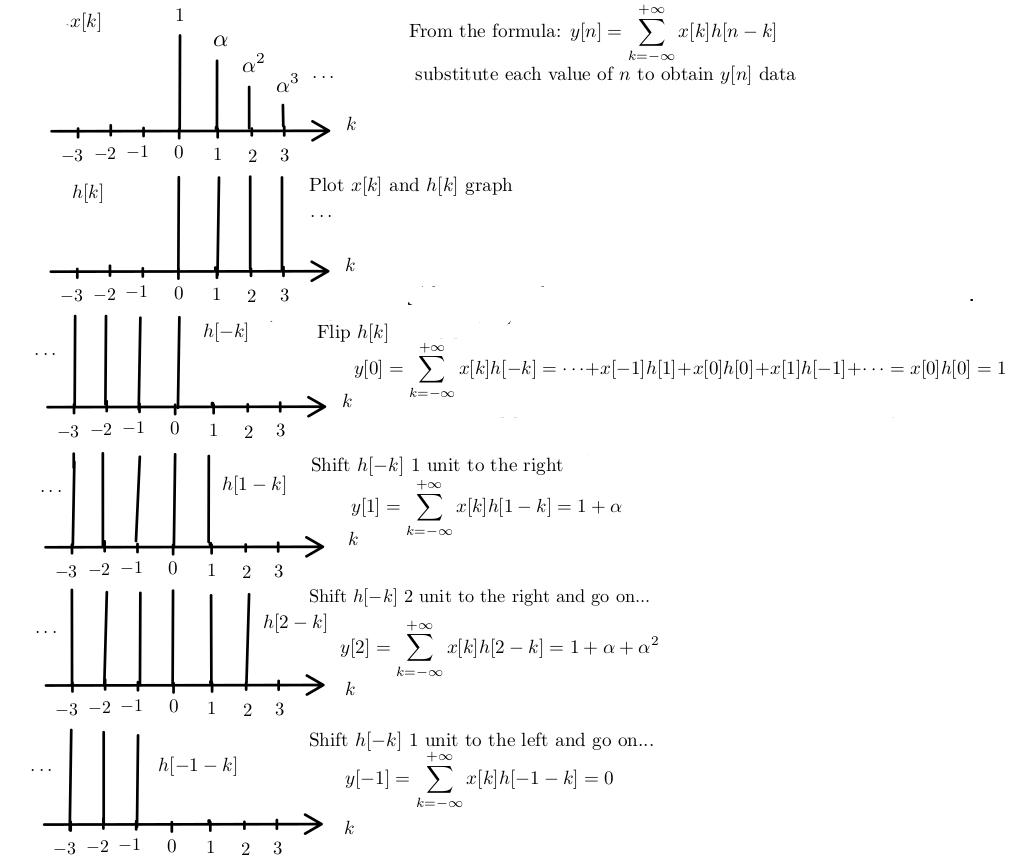
\includegraphics[width=0.8\textwidth]{conv.jpg}
			\caption{Perform convolution step by step}\label{fig:re4}
		\end{figure}
\end{frame}
\begin{frame}{Biểu diễn hệ thống LTI bằng đáp ứng xung}
Tổng quát hóa, nếu ta dịch $h[-k]$ đi $n$ đơn vị ($n$ không âm) thì:
$$y[n]=\sum_{k=-\infty}^{+\infty}x[k]h[n-k]=1+\alpha+\alpha^2+...+\alpha^n=\frac{1-\alpha^{n+1}}{1-\alpha}$$
Vậy ta thu được tín hiệu ra: $$y[n]=\frac{1-\alpha^{n+1}}{1-\alpha}u[n]=\frac{1}{1-\alpha}u[n]$$
Suy ngẫm: tại sao $h[1-k]$ lại là phiên bản \alert{dịch phải} của $h[-k]$ ? Giải thích câu trả lời của bạn.
\\ Đào sâu hơn một chút, từ công thức tính tích chập tổng quát:
$$y[n]=\sum_{k=-\infty}^{+\infty}x[k]h[n-k]=\alert{x[n]*h[n]}$$
Ta đặt $n-k=m$, dễ thấy:
$$y[n]=\sum_{m=+\infty}^{-\infty}x[n-m]h[m]=\sum_{m=-\infty}^{+\infty}x[n-m]h[m]=\alert{h[n]*x[n]}$$
Vậy ta kết luận \textbf{tích chập có tính giao hoán}.
\end{frame}
\begin{frame}{Biểu diễn hệ thống LTI bằng đáp ứng xung}
Suy ngẫm: hãy nghiệm lại tính chất giao hoán của tích chập qua bài toán tìm đầu ra của hệ thống LTI rời rạc có đáp ứng xung $h[n]=\alpha^n u[n]$ với $0<\alpha<1$ có đầu vào là xung đơn vị nhảy bậc $x[n]=u[n]$ (unit step response). Trong quá trình tính tích chập, bạn có để ý thấy "cái gì" đang "chạy" không ?
\subsubsection{Tính chất của tích chập rời rạc}
\begin{itemize}
	\item[-] Tính chất của tích chập rời rạc
\end{itemize}
\begin{block}{Tính chất của tích chập rời rạc}
	Giao hoán: $h_{1}[n]*h_{2}[n]=h_{2}[n]*h_{1}[n]$\\
	Phân phối: $h_{1}[n]*(h_{2}[n]+h_{3}[n])=h_{1}[n]*h_{2}[n]+h_{1}[n]*h_{3}[n]$\\
	Kết hợp: $(h_{1}[n]*h_{2}[n])*h_{3}[n]=h_{1}[n]*(h_{2}[n]*h_{3}[n])$
\end{block}
Suy ngẫm: các bạn hãy thử tự mình chứng minh lại $3$ tính chất trên. Gợi ý: đặt $h[n]=h_{2}[n]+h_{3}[n]$ làm ẩn phụ. Tính chất kết hợp tương đối khó chứng minh, nhưng có thể thử theo hướng sau (optional):
\begin{equation*}
	\begin{split}
		(h_{1}[n]*h_{2}[n])*h_{3}[n]&=\sum_{m=-\infty}^{+\infty}\left(\sum_{k=-\infty}^{+\infty}h_{1}[k]h_{2}[m-k]\right)h_{3}[n-m]\\
					    &=\sum_{k=-\infty}^{+\infty}\left(\sum_{m=-\infty}^{+\infty}h_{2}[m-k]h_{3}[n-m]\right)h_{1}[k]\\
					    &=h_{1}[n]*(h_{2}[n]*h_{3}[n])\\
	\end{split}
\end{equation*}
\end{frame}
\begin{frame}{Biểu diễn hệ thống LTI bằng đáp ứng xung}
\begin{itemize}
	\item[-] Khảo sát tính chất hệ thống LTI rời rạc
\end{itemize}
\subsubsection{Khảo sát tính chất của hệ thống LTI rời rạc}
 Do các hệ thống LTI rời rạc đã có sẵn tính chất \textbf{tuyến tính} và \textbf{bất biến}, nên ta chỉ cần khảo sát $3$ tính chất còn lại gồm: \alert{không nhớ}, \alert{nhân quả} và \alert{ổn định}. Một hệ thống LTI bất kỳ có thể được biểu diễn qua phép tính tích chập như sau:
 \begin{equation*}
	 \begin{split}
		 y[n]&=x[n]*h[n]=\sum_{k=-\infty}^{+\infty}x[k]h[n-k]=\sum_{k=-\infty}^{+\infty}x[n-k]h[k] \text{     (commutative property)}\\
		     &=\dots+x[n-2]h[2]+x[n-1]h[1]+x[n]h[0]+x[n+1]h[-1]+x[n+2]h[-2]+\dots \\
	\end{split}
\end{equation*}
Quan sát đầu vào-ra của hệ thống, rất hiển nhiên ta có thể nhận ra ngay để hệ thống này \alert{không nhớ} thì tất cả các hạng tử khác $x[n]h[0]$ phải bằng $0$ (các bạn có thể xem lại lý thuyết phần \alert{Hệ thống} của \alert{Chương 1} nếu cần). Vậy ta suy ra $h[n]=0 \;(\forall n\neq 0 )$
\\ Tương tự, để hệ thống này \alert{nhân quả} thì tất cả các hạng tử lớn hơn $n$ (tương lai của thời điểm $n$) như $x[n+1]h[-1],x[n+2]h[-2],\dots$ phải bằng $0$. Vậy ta suy ra $h[n]=0\;(\forall n\leq0)$.
\\ Để hệ thống này \alert{ổn định}, ta tạo ràng buộc $|x[n]|<B$, lúc này ta có:
\begin{equation*}
\begin{split}
	|y[n]|=|x[n]*h[n]|=\left|\sum_{k=-\infty}^{+\infty}x[k]h[n-k]\right|<\sum_{k=-\infty}^{+\infty}\left|x[k]h[n-k]\right|&<B\sum_{k=-\infty}^{+\infty}|h[n-k]| \\
	      &= B\sum_{n=-\infty}^{+\infty}|h[n]|\\
\end{split}
\end{equation*}
\end{frame}
\begin{frame}{Biểu diễn hệ thống LTI bằng đáp ứng xung}
	Vậy để hệ thống \alert{ổn định}, ta suy ra: $$\sum_{n=-\infty}^{+\infty}|h[n]|<+\infty$$
	\begin{block}{Tính chất hệ thống LTI rời rạc}
Không nhớ: $h[n]=0\;(\forall n \neq 0)$\\
Nhân quả: $h[n]=0\;(\forall n\leq0)$\\
Ổn định: 
$$\sum_{n=-\infty}^{+\infty}|h[n]|<+\infty$$
\end{block}
Suy ngẫm: hệ thống LTI rời rạc có đáp ứng xung $h[n]=u[n]$ có những tính chất nào ? Nếu hệ thống này \textbf{không ổn định}, bạn hãy tìm một ví dụ để chứng minh điều đó.
\end{frame}
\begin{frame}{Biểu diễn hệ thống LTI bằng đáp ứng xung}
\subsection{Hệ thống LTI liên tục}
\begin{itemize}
	\item Hệ thống LTI liên tục
\end{itemize}
\subsubsection{Tích chập liên tục}
\begin{itemize}
	\item[-] Tích chập liên tục
\end{itemize}
Phần chứng minh công thức tích chập liên tục tương đối khó nên các bạn có thể bỏ qua (optional) và xem thẳng đến slide công thức.

\begin{figure}[h]
			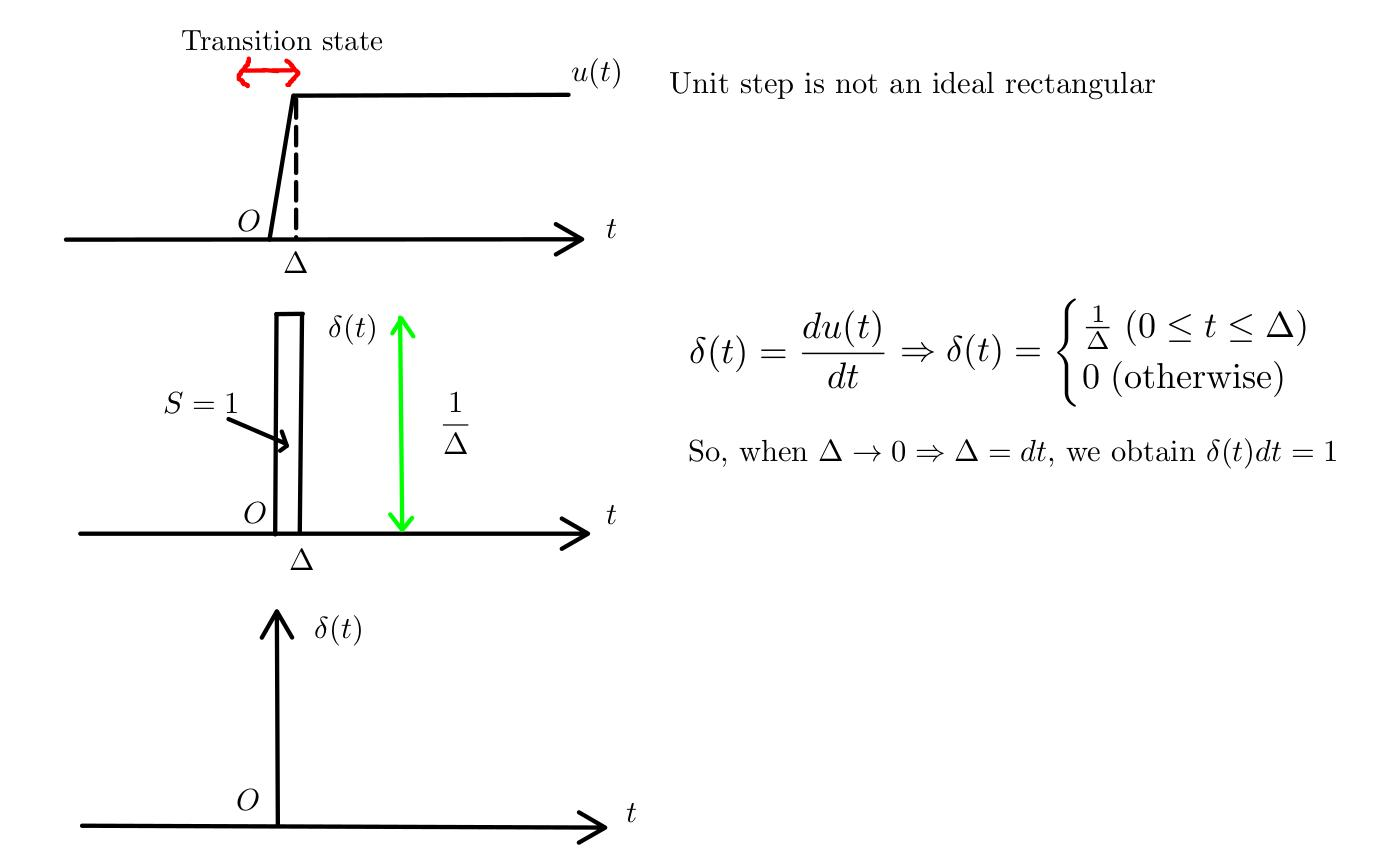
\includegraphics[width=0.9\textwidth]{dirac.jpg}
			\caption{Go deeper into Dirac impulse}\label{fig:re5}
		\end{figure}
\end{frame}
\begin{frame}{Biểu diễn hệ thống LTI bằng đáp ứng xung}
\begin{figure}[h]
			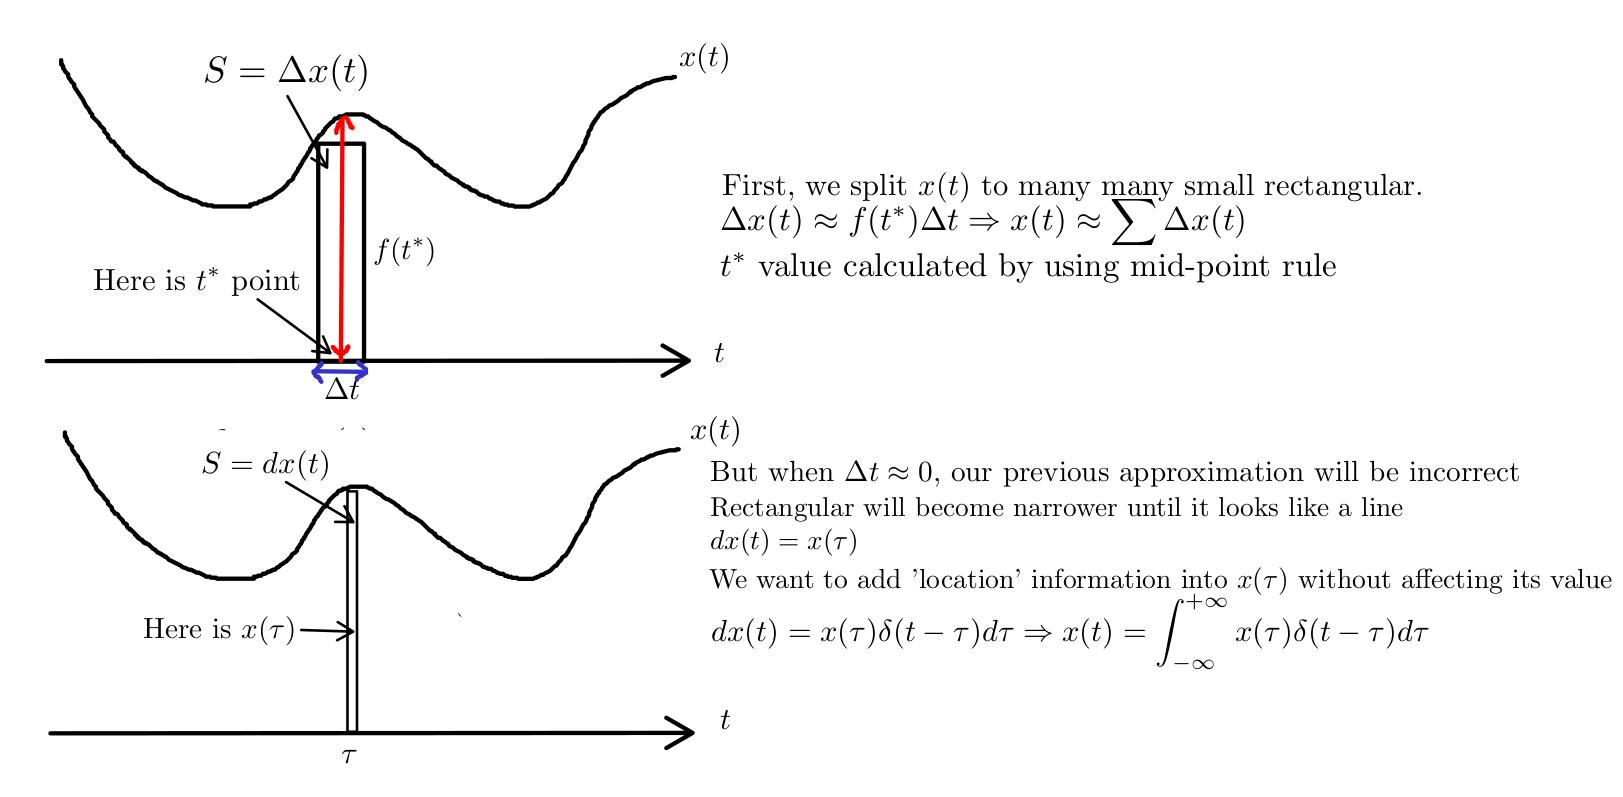
\includegraphics[width=1\textwidth]{tau.jpg}
			\caption{Represent $x(t)$ in integral form}\label{fig:re6}
		\end{figure}
\end{frame}
\begin{frame}{Biểu diễn hệ thống LTI bằng đáp ứng xung}
Tương tự như hệ thống LTI rời rạc đã trình bày ở trên, khi ta cho tín hiệu đầu vào $x(t)$ đi qua hệ thống LTI liên tục có đáp ứng xung $h(t)$, ta thu được tín hiệu đầu ra $y(t)$ có công thức như sau:
\begin{block}{Công thức biểu diễn tín hiệu $x(t)$ và $y(t)$ tổng quát}
	\begin{equation*}
	\begin{split}
		x(t)&=\int_{-\infty}^{+\infty}x(\tau)\delta(t-\tau)d\tau\\
		y(t)&=\int_{-\infty}^{+\infty}x(\tau)h(t-\tau)d\tau=\alert{x(t)*h(t)}\\
	\end{split}
	\end{equation*}
\end{block}
Ví dụ: cho tín hiệu đầu vào $x(t)=e^{-at}u(t)\; (a>0)$ qua hệ thống LTI liên tục có đáp ứng xung $h(t)=u(t)$, hãy xác định tín hiệu đầu ra $y(t)$ của hệ thống.
\end{frame}
\begin{frame}{Biểu diễn hệ thống LTI bằng đáp ứng xung}

\begin{figure}[h]
			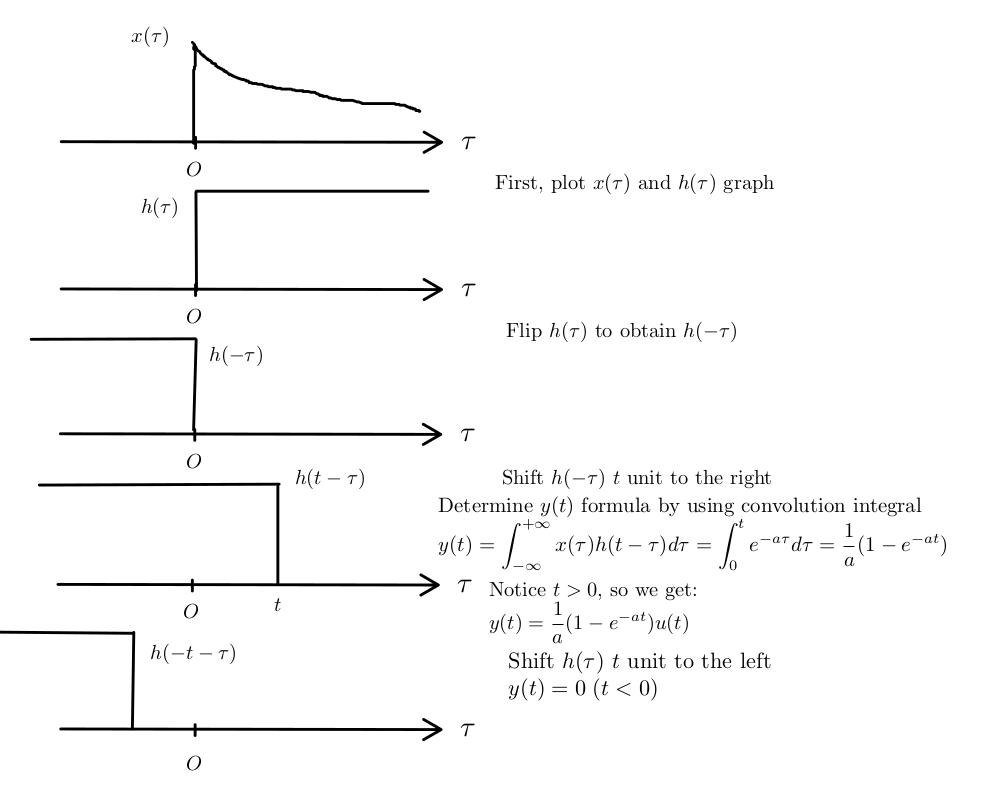
\includegraphics[width=0.8\textwidth]{conv1.jpg}
			\caption{Perform integral convolution step by step}\label{fig:re7}
		\end{figure}
\end{frame}
\begin{frame}{Biểu diễn hệ thống LTI bằng đáp ứng xung}
\subsubsection{Tính chất của tích chập liên tục}
Suy ngẫm: từ $2$ kết quả thu được của phép tính tích chập rời rạc và liên tục ở trên, các bạn hãy thử chọn một giá trị $a>0$ tùy ý rồi "ép" $\alpha=e^{-a}$, sau đó thử dùng các công cụ như Matlab/Octave (hoặc Casio tay) để phác họa dạng đồ thị của $y[n]$ và $y(t)$.

\begin{figure}[h]
			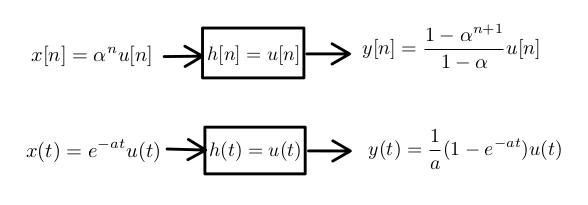
\includegraphics[width=0.6\textwidth]{result.jpg}
			\caption{Discrete and continuous time system}\label{fig:re9}
		\end{figure}
\begin{itemize}
	\item[-] Tính chất của tích chập liên tục
\end{itemize}
\begin{block}{Tính chất của tích chập liên tục}
	Giao hoán: $h_{1}(t)*h_{2}(t)=h_{2}(t)*h_{1}(t)$\\
	Phân phối: $h_{1}(t)*(h_{2}(t)+h_{3}(t))=h_{1}(t)*h_{2}(t)+h_{1}(t)*h_{3}(t)$\\
	Kết hợp: $(h_{1}(t)*h_{2}(t))*h_{3}(t)=h_{1}*(h_{2}(t)*h_{3}(t))$\\
\end{block}
Suy ngẫm: các bạn hãy thử tự mình chứng minh lại $3$ tính chất trên. Bạn có để ý thấy \textbf{điểm tương đồng} trong cách sử dụng phép toán tích phân và tổng vô hạn không ? Điểm tương đồng này giúp bạn hiểu sâu hơn bản chất về mối liên hệ giữa "miền tương tự" và "miền rời rạc" như thế nào (gợi ý: tham khảo ý tưởng của tổng Riemann) ?
\end{frame}
\begin{frame}{Biểu diễn hệ thống LTI bằng đáp ứng xung}
\begin{figure}[h]
			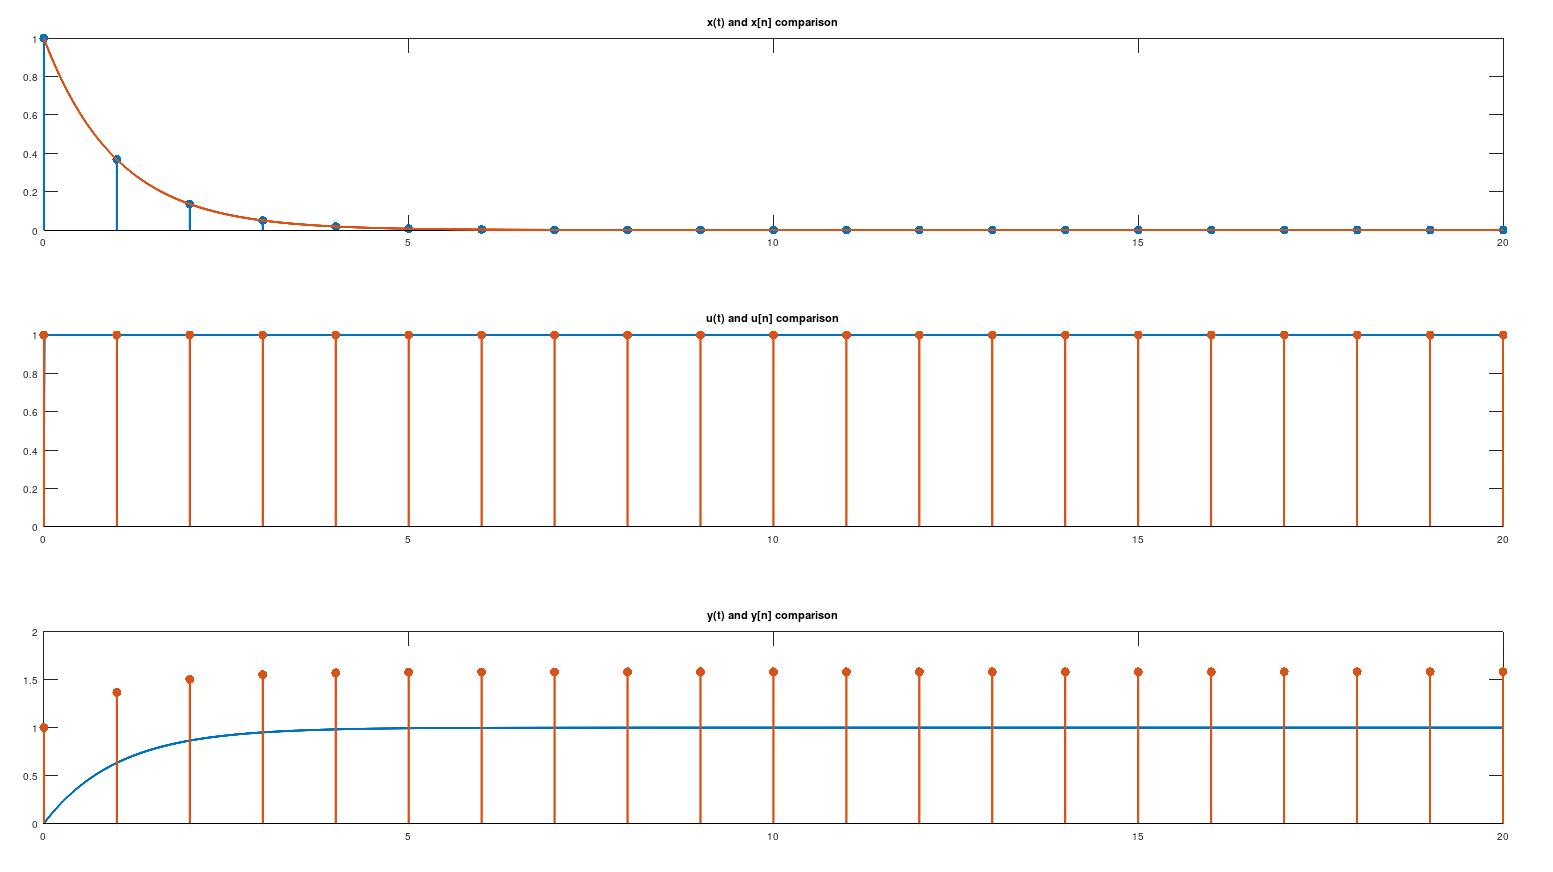
\includegraphics[width=1\textwidth]{test.jpg}
			\caption{Does this graph $(a=1)$ make any sense ? Can you feel something behind it ?}\label{fig:re10}
		\end{figure}
\end{frame}
\begin{frame}{Biểu diễn hệ thống LTI bằng đáp ứng xung}
\subsubsection{Khảo sát tính chất của hệ thống LTI liên tục}
\begin{itemize}
	\item[-] Khảo sát tính chất của hệ thống LTI liên tục
\end{itemize}
	Với ý tưởng hoàn toàn tương tự như khảo sát tính chất của hệ thống LTI rời rạc như ở trên, ta cũng xem xét $3$ tính chất của hệ thống gồm \alert{tính không nhớ}, \alert{tính nhân quả}, \alert{tính ổn định}. Từ công thức xác định đầu ra của hệ thống LTI tương tự, ta có:
	$$y(t)=\int_{-\infty}^{+\infty}x(\tau)h(t-\tau)d\tau=\int_{-\infty}^{+\infty}x(t-\tau)h(\tau)d\tau$$
Hiển nhiên ta có thể thấy ngay:
\begin{enumerate}
	\item Hệ thống không nhớ khi và chỉ khi $h(\tau)=0\;(\forall \tau\neq 0)$
	\item Hệ thống nhân quả khi và chỉ khi $h(\tau)=0\;(\forall \tau\leq0)$
	\item Hệ thống ổn định khi và chỉ khi:
\begin{equation*}
\begin{split}
	|y(t)|&=\left|\int_{-\infty}^{+\infty}x(t-\tau)h(\tau)d\tau\right|<\int_{-\infty}^{+\infty}|x(t-\tau)h(\tau)|d\tau<B\int_{-\infty}^{+\infty}|h(\tau)|d\tau<+\infty\\
&\Leftrightarrow \int_{-\infty}^{+\infty}|h(\tau)|d\tau<+\infty
\end{split}
\end{equation*}
\end{enumerate}
\end{frame}
\begin{frame}{Biểu diễn hệ thống LTI bằng đáp ứng xung}
	\begin{block}{Tính chất của hệ thống LTI liên tục}
		Không nhớ: $h(t)=0\;(\forall t\neq 0)$\\

		Nhân quả: $h(t)=0\;(\forall t\leq 0)$\\

		Ổn định:
$$\int_{-\infty}^{+\infty}|h(t)|dt<+\infty$$
	\end{block}
Suy ngẫm: sau khi đã hiểu bản chất phép toán tích chập, bạn hãy lý giải tại sao đây là hệ thống LTI ?
\begin{equation*}
	\begin{split}
		y[n]&=x[n]*h[n]\\
		y(t)&=x(t)*h(t)\\
	\end{split}
\end{equation*}
\end{frame}
\begin{frame}{Biểu diễn hệ thống LTI bằng phương trình đầu vào-ra}
\section{Biểu diễn hệ thống LTI bằng phương trình đầu vào-ra}
\subsection{Hệ thống LTI liên tục}
\subsubsection{Ôn tập phương trình vi phân (optional)}
\begin{itemize}
	\item Hệ thống LTI liên tục
	\end{itemize}
\begin{itemize}
\item[-] Ôn tập phương trình vi phân (optional)
\end{itemize}
Phương trình vi phân tổng quát có dạng như sau:
$$\sum_{k=0}^{M}a_{k}\frac{dy^k(t)}{dt^k}=\sum_{k=0}^{N}b_{k}\frac{dx^k(t)}{dt^k}$$
Giải phương trình vi phân (còn gọi là phương trình ODE - Ordinary Differential Equation) tức là tìm phương trình của hàm $y(t)$ tương ứng với mỗi hàm $x(t)$ cho trước. Người ta đã chứng minh được nghiệm của phương trình vi phân bất kì có công thức tổng quát (general solution) như sau:
$$y_{G}(t)=y_{P}(t)+y_{H}(t)$$
Các nghiệm của phương trình vi phân được tìm ra như sau:
\begin{enumerate}
	\item Nghiệm $y_{P}(t)$: là nghiệm riêng (particular solution) của phương trình ODE, được tính khi thay thẳng $x(t)$ vào giải phương trình vi phân.
	\item Nghiệm $y_{H}(t)$: là nghiệm thuần nhất (homogeneous solution) của phương trình ODE, được tính khi thay \alert{$x(t)=0$} vào giải phương trình vi phân.
	\item Nghiệm $y_{G}(t)$: là nghiệm tổng quát (general solution) của phương trình ODE, được tính theo công thức trên. Tùy thuộc vào điều kiện khởi tạo (intial condition) của phương trình, ta thay nốt hệ điều kiện vào $y_{G}(t)$ để tìm ra đáp án cuối cùng.
\end{enumerate}
\end{frame}
\begin{frame}{Biểu diễn hệ thống LTI bằng phương trình đầu vào-ra}
Ví dụ: giải phương trình vi phân đơn giản với điều kiện $y(0)=5$:
$$\frac{dy(t)}{dt}+4y(t)=3t$$
Ta tiến hành giải các nghiệm theo 3 bước như trên:
\begin{enumerate}
	\item Nghiệm $y_{P}(t)$: ta đoán dạng nghiệm $y_{P}(t)=at+b$, thay vào phương trình ta thu được: $$a+4at+4b=3t$$
Đồng nhất các hệ số, ta thu được $a,b$ và nghiệm $y_{P}(t)$ như sau:
$$y_{P}(t)=\frac{3}{4}t-\frac{3}{16}$$
\item Nghiệm $y_{H}(t)$: ta đoán dạng nghiệm $y_{H}(t)=Ke^{\lambda t}$, thay vào phương trình thuần nhất $x(t)=0$, ta có:
	$$K\lambda e^{\lambda t}+4K e^{\lambda t}=0$$
Đồng nhất các hệ số, ta thu được $\lambda=-4$ và nghiệm $y_{H}(t)$ như sau:
$$y_{H}(t)=\alert{K}e^{-4t}$$
\item Nghiệm $y_{G}(t)$: từ hai nghiệm đã tìm được ở trên, ta thu được dạng nghiệm $y_{G}(t)$ như sau:
	$$y_{G}(t)=y_{P}(t)+y_{H}(t)=\frac{3}{4}t-\frac{3}{16}+\alert{K}e^{-4t}$$
	Thay nốt điều kiện đầu $y(0)=5$, ta tìm ra được $K=\frac{83}{16}$. 
\end{enumerate}
\end{frame}
\begin{frame}{Biểu diễn hệ thống LTI bằng phương trình đầu vào-ra}
\begin{itemize}
	\item[-] Sử dụng phương trình vi phân phân tích hệ thống LTI liên tục  
\end{itemize}
\subsubsection{Sử dụng phương trình vi phân phân tích hệ thống LTI liên tục}

Một hệ thống LTI liên tục không chỉ có thể được biểu diễn trực tiếp bằng \textbf{đáp ứng xung} mà còn có thể được biểu diễn gián tiếp thông qua \textbf{phương trình đầu vào-ra}. Xét một hệ thống LTI được biểu diễn như sau:

$$\sum_{k=0}^{M}a_{k}\frac{dy^k(t)}{dt^k}=\sum_{k=0}^{N}b_{k}\frac{dx^k(t)}{dt^k}$$
với các điều kiện khởi tạo $y(0)$, $y'(0)$,... là các hằng số.
\\Suy ngẫm (khó): tại sao hệ thống trên là hệ thống LTI ? Gợi ý, nếu bạn chưa giải thích được cho trường hợp hệ thống tổng quát thì hãy thử tìm phương trình đầu vào-ra của hệ thống bậc 1 rất đơn giản sau (dùng Euler's trick để tìm mối quan hệ giữa $y(t)$ và $x(t)$):
$$\frac{dy(t)}{dt}+y(t)=x(t)$$
\end{frame}
\begin{frame}{Biểu diễn hệ thống LTI bằng phương trình đầu vào-ra}
Trước khi đi sâu vào phân tích công thức, ta hãy quan sát hiện tượng ấn nút nguồn (power) để khởi động một chiếc máy tính. Máy tính lúc đầu sẽ hiện trạng thái boot system mất khoảng vài giây (tùy từng dòng máy) sau đó mới mở giao diện hệ điều hành ở trạng thái ổn định. Hoặc ta quan sát quá trình thang máy hoạt động chẳng hạn, khi khởi động thang máy luôn mất một khoảng thời gian ngắn để gia tốc từ trạng thái đứng yên đến khi vận tốc thang ổn định.
\\ Từ quan sát này, ta có thể thấy khi tác động tín hiệu input bất kì vào hệ thống (như ấn nút nguồn máy tính hay ấn nút thang máy), hệ thống luôn \textbf{mất một khoảng thời gian rất ngắn chuyển tiếp giữa trạng thái tĩnh (không hoạt động) đến trạng thái hoạt động ổn định}. Ta có thể nhận thấy tín hiệu output của hệ thống gồm 2 thành phần gồm \alert{đáp ứng của hệ thống trạng thái chuyển tiếp} và \alert{đáp ứng của hệ thống trạng thái ổn định}.


\begin{figure}[h]
			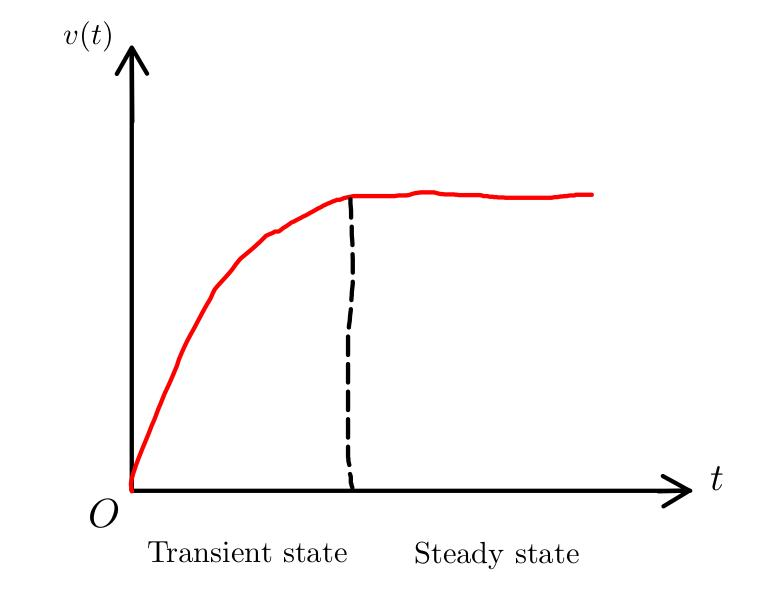
\includegraphics[width=0.4\textwidth]{elevator.jpg}
			\caption{Elevator velocity graph }\label{fig:re11}
		\end{figure}
\end{frame}
\begin{frame}{Biểu diễn hệ thống LTI bằng phương trình đầu vào-ra}
	Từ quan sát hiện tượng vật lý thực tiễn như trên, ta xây dựng công thức đáp ứng hệ thống tổng quát $y_{T}(t)$ (total response) như sau:
	$$y_{T}(t)=y_{N}(t)+y_{F}(t)$$
với các nghiệm gồm:
\begin{enumerate}
	\item Nghiệm $y_{N}(t)$: là đáp ứng tự nhiên (natural response) của hệ thống. Đây là đáp ứng của hệ thống ở trạng thái chuyển tiếp (transient state) giữa trạng thái tĩnh và hoạt động ổn định. Từ nhận định này ta có thể thấy đây chính là \alert{nghiệm thuần nhất $y_{H}(t)$} của phương trình ODE, với  hệ các \textbf{điều kiện khởi tạo $y(0), y'(0), y''(0),..$}.
	\item Nghiệm $y_{F}(t)$: là đáp ứng cưỡng bức (forced response) của hệ thống. Đây là đáp ứng của hệ thống ở trạng thái ổn định (steady state). Từ nhận định này ta có thể thấy đây chính là \alert{nghiệm tổng quát $y_{G}(t)$} của phương trình ODE, với hệ các \textbf{điều kiện khởi tạo bằng 0}.
	\item Nghiệm $y_{T}(t)$: là đáp ứng hệ thống (total response) được tính theo công thức trên.
\end{enumerate}
\end{frame}
\begin{frame}{Biểu diễn hệ thống LTI bằng phương trình đầu vào-ra}
Ví dụ: cho hệ thống LTI liên tục được biểu diễn như sau với điều kiện khởi tạo $y(0)=5$
$$\frac{dy(t)}{dt}+4y(t)=x(t)$$
Tìm đầu ra của hệ thống với đầu vào $x(t)=3tu(t)$.
\\ Ta tiến hành giải các nghiệm (các đáp ứng hệ thống) theo 3 bước như trên:
\begin{enumerate}
	\item Nghiệm $y_{N}(t)$: với \alert{$x(t)=0$}, giải với quy trình như ở trên, ta tìm được: $$y_{N}(t)=Ke^{-4t}$$
Với điều kiện khởi tạo $y(0)=5$, ta dễ dàng tìm được $K=5$.
	\item Nghiệm $y_{F}(t)$: với $x(t)=3tu(t)$, giải với quy trình như ở trên, ta tìm được:
		$$y_{F}(t)=\frac{3}{4}t-\frac{3}{16}+Ce^{-4t}$$
		Với điều kiện \alert{$y(t)=0$}, ta tìm được $C=\frac{3}{16}$
	\item Nghiệm $y_{T}(t)$, ta dễ dàng tìm được:
		$$y_{T}(t)=y_{N}(t)+y_{F}(t)=\frac{3}{4}t-\frac{3}{16}+\frac{83}{16}e^{-4t}$$
\end{enumerate}
\alert{\textit{Lưu ý: đáp ứng cưỡng bức của hệ thống có dạng của nghiệm tổng quát chứ không phải nghiệm riêng.}}
\\Suy ngẫm: theo bạn, trong hai cách tìm đáp ứng hệ thống bằng phương trình vi phân đã được trình bày ở trên, cách nào giúp bạn hiểu trực quan và sâu sắc về hành vi của hệ thống hơn ? 
\end{frame}
\begin{frame}{Biểu diễn hệ thống LTI bằng phương trình đầu vào-ra}
\subsection{Hệ thống LTI rời rạc}
\begin{itemize}
	\item Hệ thống LTI rời rạc
\end{itemize}
\subsubsection{Ôn tập phương trình sai phân (optional but recommended)}
\begin{itemize}
	\item[-] Ôn tập phương trình sai phân (optional but recommended)
\end{itemize}
Phương trình sai phân có dạng tổng quát như sau:
$$\sum_{k=0}^{M}a_{k}y[n-k]=\sum_{k=0}^{N}b_{k}x[n-k]$$
Tương tự như nghiệm phương trình vi phân ODE, nghiệm của phương trình sai phân DE (Difference Equation) có dạng: $$y_{G}[n]=y_{P}[n]+y_{H}[n]$$
Các nghiệm của phương trình sai phân được tìm ra như sau:
\begin{enumerate}
	\item Nghiệm $y_{P}[n]$: là nghiệm riêng (particular solution) của phương trình DE, được tính khi thay thẳng $x[n]$ vào phương trình sai phân.
	\item Nghiệm $y_{H}[n]$: là nghiệm thuần nhất (homogeneous solution) của phương trình DE, được tính khi thay \alert{$x[n]=0$} vào phương trình sai phân.
	\item Nghiệm $y_{G}[n]$: là nghiệm tổng quát (general solution) của phương trình DE, được tính theo công thức ở trên. Tùy vào điều kiện khởi tạo (initial condition) của phương trình, ta thay nốt hệ điều kiện vào $y_{G}[n]$ để tìm ra đáp án cuối cùng.
\end{enumerate}
\end{frame}
\begin{frame}{Biểu diễn hệ thống LTI bằng phương trình đầu vào-ra}
Ví dụ: giải phương trình sai phân đơn giản với điều kiện $y[0]=5$:
$$y[n]-3y[n-1]=4n$$
Ta tiến hành giải các nghiệm theo 3 bước như trên:
\begin{enumerate}
	\item Nghiệm $y_{P}[n]$: ta đoán dạng nghiệm $y[n]=an+b$, thay vào phương trình ta thu được: 
	\begin{equation*}
	\begin{split}
		y[n]&=3y[n-1]+4n\\
		\Leftrightarrow an+b&=3[a(n-1)+b]+4n \\
		\Leftrightarrow an+b&=(3a+4)n-(3a-3b)\\
	\end{split}
	\end{equation*}
	Đồng nhất hệ số, ta thu được $a=-2\, , b=-3$. Vậy ta thu được nghiệm riêng $y_{P}[n]=-2n-3$.
\item Nghiệm $y_{H}[n]$: ta dễ dàng thấy ngay sau khi thay \alert{$x[n]=0$}, phương trình sai phân trở thành một \textbf{cấp số nhân}: $$y[n]=3y[n-1]$$
	Vậy ta thu được nghiệm thuần nhất của phương trình DE là $y_{H}[n]=K3^{n}$.
\item Nghiệm $y_{G}[n]$: ta tìm được dạng nghiệm tổng quát như sau: $$y_{G}[n]=y_{P}[n]+y_{H}[n]=-2n-3+K3^n$$
Thay nốt điều kiện đầu $y[0]=5$, ta tìm được $K=8$.
\end{enumerate}
\end{frame}
\begin{frame}{Biểu diễn hệ thống LTI bằng phương trình đầu vào-ra}
\begin{itemize}
\item[-] Sử dụng phương trình sai phân phân tích hệ thống LTI rời rạc
\end{itemize}
\subsubsection{Sử dụng phương trình sai phân phân tích hệ thống LTI rời rạc}
 Hệ thống LTI rời rạc tổng quát có thể được biểu diễn qua phương trình sai phân sau:
$$\sum_{k=0}^{M}a_{k}y[n-k]=\sum_{k=0}^{N}b_{k}x[n-k]$$
\\ Suy ngẫm (khó): tại sao hệ thống trên là hệ thống LTI ? Nếu bạn chưa chứng minh được trường hợp tổng quát, hãy thử xét một trường hợp cụ thể sau: 
$$y[n]=y[n-1]+x[n]$$
Tương tự như hệ thống LTI liên tục, ta xây dựng công thức đáp ứng hệ thống tổng quát $y_{T}[n]$ (total response) như sau: $$y_{T}[n]=y_{N}[n]+y_{F}[n]$$
với các nghiệm gồm:
\begin{enumerate}
	\item Nghiệm $y_{N}[n]$: là đáp ứng tự nhiên (natural response) của hệ thống. Đây chính là \alert{nghiệm thuần nhất $y_{H}[n]$} của phương trình DE, với hệ các \textbf{điều kiện khởi tạo $y[0]\; ,y[-1]\; ,y[-2],...$}
	\item Nghiệm $y_{F}[n]$: là đáp ứng cưỡng bức (forced response) của hệ thống. Đây chính là \alert{nghiệm tổng quát $y_{G}[n]$} của phương trình DE, với hệ các \textbf{điều kiện khởi tạo bằng 0.}
	\item Nghiệm $y_{T}[n]$: là đáp ứng hệ thống (total response) được tính theo công thức trên.
\end{enumerate}
\end{frame}
\begin{frame}{Biểu diễn hệ thống LTI bằng phương trình đầu vào-ra}
Ví dụ: hệ thống LTI rời rạc được biểu diễn như sau với điều kiện khởi tạo $y[0]=5$
$$y[n]-3y[n-1]=4n$$
Tìm đầu ra của hệ thống với đầu vào $x[n]=4nu[n]$.
Ta tiến hành giải các nghiệm (các đáp ứng hệ thống) theo 3 bước như trên:
\begin{enumerate}
	\item Nghiệm $y_{N}[n]$: với \alert{$x[n]=0$}, giải với quy trình như ở trên, ta tìm được: $$y_{N}[n]=K3^{n}$$
		Với điều kiện khởi tạo $y[0]=5$, ta dễ dàng tính được giá trị $K=5$.
	\item Nghiệm $y_{F}[n]$: với $x[n]=4nu[n]$, giải nghiệm tổng quát (general solution) với quy trình như ở trên, ta tìm được:
		$$y_{F}[n]=-2n-3+C3^n$$
	Với điều kiện \alert{$y[0]=0$}, ta tìm được $C=3$.
\item Nghiệm $y_{T}[n]$, ta dễ dàng tìm được:
	$$y_{T}[n]=y_{N}[n]+y_{F}[n]=-2n-3+8.3^n$$
\end{enumerate}
	Suy ngẫm: khi phân tích hệ thống LTI với một góc nhìn khác, ta gọi hai đáp ứng lối ra là $y_{zs}[n]$ (zero-state response) và $y_{zi}[n]$ (zero-input response). Theo bạn, chúng tương ứng với các nghiệm nào ($y_{F}[n]\; ,y_{N}[n]$) ? Hãy giải thích câu trả lời của bạn. 
\end{frame}
\end{document}

